% -*- LaTeX -*-
% -*- coding: utf-8 -*-
%
% michael a.g. aïvázis
% california institute of technology
% (c) 1998-2012 all rights reserved
%

\documentclass[12pt,answers]{exam}

% packages, setup, macros, etc.
% -*- LaTeX -*-
% -*- coding: utf-8 -*-
%
% ~~~~~~~~~~~~~~~~~~~~~~~~~~~~~~~~~~~~~~~~~~~~~~~~~~~~~~~~~~~~~~~~~~~~~~~~~~~~~~
%
%                             michael a.g. aïvázis
%                      california institute of technology
%                      (c) 1998-2010  all rights reserved
%
% ~~~~~~~~~~~~~~~~~~~~~~~~~~~~~~~~~~~~~~~~~~~~~~~~~~~~~~~~~~~~~~~~~~~~~~~~~~~~~~
%


% language
\usepackage[english]{babel}

% beamer configuration
\usepackage{acm114}

% typesetting interactive sessions
\usepackage{fancyvrb}

% dimensions
\usepackage{fancyhdr}

% fonts
\usepackage{amsfonts}
\usepackage{times}
%\usepackage[iso-8859-7]{inputenc}

% figures
\usepackage{graphicx}
\definecolor{acm114@cream}{rgb}{0.96, .95, .89}
\definecolor{acm114@sand}{rgb}{0.86, .85, .77}
\definecolor{acm114@stone}{rgb}{0.55, .54, .46}
\definecolor{acm114@leather}{rgb}{0.48, .47, .38}
\definecolor{acm114@olive}{rgb}{0.28, .29, .25}
\definecolor{acm114@lava}{rgb}{0.25, .23, .22}


% listings and their configurations
\usepackage[slide,algoruled,linesnumbered,noend]{algorithm2e}
\SetKwComment{tnm}{\#}{}
\SetKw{KwAnd}{and}
\SetKw{KwSend}{send}
\SetKw{KwRecv}{recv}
\SetKw{KwFrom}{from}

\usepackage{subfigure}
\usepackage{textcomp}

\usepackage{listings}
\lstloadlanguages{C,C++,python,bash}
\lstset{
  columns=flexible,
  upquote=true,
  % 
  aboveskip=\medskipamount,
  belowskip=\smallskipamount,
  % 
  numbers=left,
  numberstyle=\color{acm114@stone}\tiny,
  stepnumber=1,
  numbersep=5pt,
  numberblanklines=true,
  % 
  basicstyle=\tt\bfseries\scriptsize,
  keywordstyle=\color{acm114@leather}\bfseries,
  commentstyle=\color{acm114@stone}\slshape,
  stringstyle=\color{acm114@olive}\slshape,
  showstringspaces=false,
  % 
  frame=,
  captionpos=t,
  backgroundcolor=\color{acm114@cream},
  xleftmargin=0em,
  xrightmargin=0em
} 

\lstnewenvironment{shell}[2][]{
  \lstset{
    language=bash,
    %
    escapeinside={\#@}{@},
    %
    #1
  }}{#2}

\lstnewenvironment{python}[2][]{
  \lstset{
    language=python,
    morekeywords={self,yield,False,True,None},
    escapeinside={\#@}{@},
    %
    #1
  }}{#2}

\lstnewenvironment{C}[1][]{
  \lstset{
    language=c,
    %
    escapeinside={//@}{@},
    %
    #1
  }}{}

\lstnewenvironment{C++}[2][]{
  \lstset{
    language=C++,
    %
    escapeinside={/*}{*/},
    %
    #1
  }}{#2}

% references
\usepackage[numbers]{natbib}
\bibliographystyle{unsrtnat}
\renewcommand\bibsection{\section{\refname}}
\def\newblock{\small}

% misc
\usepackage{dcolumn}
\newcolumntype{d}[1]{D{.}{.}{#1}}

\usepackage{url}
\usepackage{hyperref}


% shortcuts
\def\slideref#1{{Slide~\ref{slide:#1}}}
\def\algref#1{{Alg.~\ref{alg:#1}}}
\def\alglineref#1{{line~\ref{line:#1}}}
\def\eqref#1{{Eq.~\ref{eq:#1}}}
\def\figref#1{{Fig.~\ref{fig:#1}}}
\def\secref#1{{Sec.~\ref{sec:#1}}}
\def\tabref#1{{Table~\ref{tab:#1}}}
\def\lstref#1{{Listing~\ref{lst:#1}}}
\def\lstlineref#1{{line~\ref{line:#1}}}

% macros
\def\href#1{{\footnotesize\bfseries\url{#1}}}
\def\defeq{\mathrel{\mathop:}=}
\def\GNU{\mbox{\tt\small GNU}}
\def\GSL{\mbox{\tt\small GSL}}
\def\RANLUX{\mbox{\tt\small RANLUX}}
\def\NULL{\mbox{\tt\small NULL}}

\def\cc{\mbox{\tt\small C}}
\def\cpp{\mbox{\tt\small C++}}
%\def\cpp{\mbox{\tt C\raise.4ex\hbox{++}}}
\def\fortran{{\tt\small FORTRAN}}
\def\f90{{\tt\small FORTRAN90}}
\def\mpi{{\tt MPI}}
\def\th#1{\mbox{$#1^{\rm th}$}}

\def\bydef{\mathrel{\mathop:}=}
\def\Li{\mbox{\rm Li}_{2}}

\def\pyre{{\tt pyre}}

\def\order#1{\mbox{$\mathcal{O}(#1)$}}
\def\class#1{\mbox{\tt #1}}
\def\component#1{\mbox{\tt #1}}
\def\function#1{\mbox{\tt #1}}
\def\method#1{\mbox{\tt #1}}
\def\identifier#1{\mbox{\tt #1}}
\def\keyword#1{\mbox{\tt #1}}
\def\operator#1{\mbox{\tt #1}}
\def\srcfile#1{\mbox{\tt #1}}

\def\insertionsort{\mbox{\sc Insertion-Sort}}
\def\mergesort{\mbox{\sc Merge-Sort}}
\def\merge{\mbox{\sc Merge}}

\def\TODO#1{{%
    \subsubsection*{Still to do}%
    \scriptsize\tt%
    \begin{list}{\leftpointright}{} #1 \end{list}}}

% set up the PDF options
\hypersetup{
    pdftitle={ACM/CS 114: Winter 2010},
    pdfauthor={Michael A.G. A\"iv\'azis},
    pdfsubject={Lecture notes},
    pdfkeywords=,           % list of keywords
%
    bookmarks=true,         % show bookmarks bar?
    unicode=false,          % non-Latin characters in Acrobat's bookmarks
    pdftoolbar=true,        % show Acrobat's toolbar?
    pdfmenubar=true,        % show Acrobat's menu?
    pdffitwindow=true,      % page fit to window when opened
    pdfnewwindow=true,      % links in new window
    colorlinks=true,        % false: boxed links; true: colored links
    linkcolor=acm114@sand,  % color of internal links
    citecolor=acm114@stone  % color of links to bibliography
    filecolor=acm114@sand,  % color of file links
    urlcolor=acm114@stone   % color of external links
}
% end of file 


\begin{document}
\pagestyle{headandfoot}
\runningfootrule
\firstpageheader{ACM/CS 114}{Assignment 1}{Due: 7 May 2012}
\runningheader{}{}{}
\firstpagefooter{}{}{}
\runningfooter{ACM/CS 114}{Assignment 1}{\thepage}

% intro
As warm up, we will repeat some of the assignments from the previous quarter, but this time you
\emph{must} implement everything in python. Answering these questions does not require
extensive familiarity with the large number of packages in the python runtime: we will only use
the package \identifier{random}. But feel free to look around.

\begin{questions}

% --------------------------------------
% merge sort
\question
Recall the pseudocode for \mergesort:
%
\begin{center}
  \begin{minipage}{.5\linewidth}
    \begin{algorithm}[H]
      \label{alg:merge-sort}
%
      \DontPrintSemicolon
      %\NoCaptionOfAlgo
      \SetAlCapHSkip{0ex}
%
      \caption{\mergesort($S$, $p$, $r$)}
      \vspace{.5em}
%
      \If{$p < r$}{
        $q \leftarrow \lfloor (p+r)/2 \rfloor$ \;
        \mergesort($S$, $p$, $q$) \;
        \mergesort($S$, $q+1$, $r$) \;
        \merge($S$, $p$, $q$, $r$) \;
      }
%
      \vspace{.5em}
%
    \end{algorithm}
  \end{minipage}
\end{center}
%
\begin{parts}
\part Implement \mergesort\ and \merge, its workhorse, in python.
\part Write a driver that invokes it with $S = (5, 2, 4, 6, 1, 3)$.
\part Build a container with $10^6$ random numbers. Sort it using your implementation.
\end{parts}

% --------------------------------------
% dilog
\def\Li{\mbox{\rm Li}_{2}}
\def\dilog{\function{dilog}}
\question Recall the definition for the dilogarithm in terms of the integral
%
\begin{equation}
\Li(z) \bydef
- \int_{0}^{z} dz' \; \frac{\log(1-z')}{z'} \label{eq:li-def}
\end{equation}
%
\begin{parts}
\part Implement a function \dilog\ that accepts a real number $z$ and an integer $N$, and
returns an approximation to \eqref{li-def} using the midpoint rule.
\part Build a table of the value, the error and the amount of time it takes to compute $\Li(1)$
and $\Li(-1)$, for $N \in \{ 10, 10^3, 10^6, 10^9 \}$.
%
\end{parts}

% --------------------------------------
% montecarlo
\question Use Monte Carlo integration to compute an approximation to the value of $\pi$ by
computing the area of the upper right quadrant of a unit circle centered at the origin, as
shown below.
%
\begin{figure}[h]
\centering
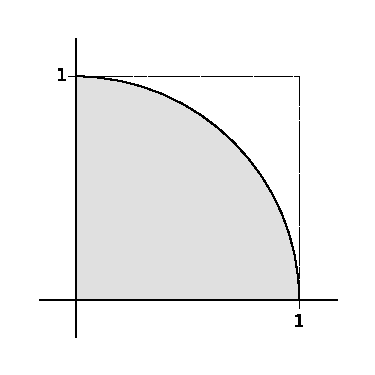
\includegraphics[scale=.5]{pie.pdf}
\end{figure}
%

\end{questions}

\end{document}

% end of file 
